

%% AAPT Physics Bowl Exams Questions
%%----------------------------------------


%% this section contains 67 problems


%% PhysicsBowl 2015
%%----------------------------------------
\element{aapt}{ %% Bowl-A3
\begin{question}{bowl-2015-q13}
    An object is being pushed at constant speed on an inclined plane.
    The free body diagram of the object is shown with the gravitational force represented by $W$,
        the friction force by $f$,
        the applied external push parallel to the incline by $F$,
        and the normal force with the surface by $n$.
    %[Vectors are not drawn to scale.] ??
    \begin{center}
    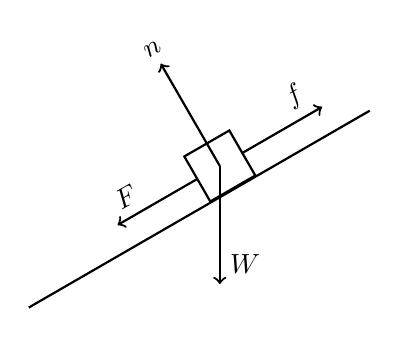
\begin{tikzpicture}
        %% Ramp
        \draw[thick] (0,0) -- (30:5cm);
        %% Box
        \node[thick,draw,rectangle,minimum size=0.66cm,rotate=30,anchor=south]
            (B) at (30:3cm) {};
        %% Arrows
        \draw[thick,->] (B) -- ++ (210:1.5cm)
            node[anchor=south west,rotate=30] {$F$};
        \draw[thick,->] (B) -- ++ (30:1.5cm)
            node[anchor=south east,rotate=30] {$f$};
        \draw[thick,->] (B.center) -- ++ (270:1.5cm)
            node[anchor=south west] {$W$};
        \draw[thick,->] (B.center) -- ++ (120:1.5cm)
            node[anchor=south,rotate=30] {$n$};
    \end{tikzpicture}
    \end{center}
    Which one of the following choices represents correct relationships between the forces?
    \begin{multicols}{2}
    \begin{choices}
        \wrongchoice{$n>W$ and $F<f$}
        \wrongchoice{$n<W$ and $F=f$}
      \correctchoice{$n<W$ and $F<f$}
        \wrongchoice{$n=W$ and $F>f$}
        \wrongchoice{$n=W$ and $F=f$}
    \end{choices}
    \end{multicols}
\end{question}
}

\element{aapt}{ %% Bowl-A3
\begin{question}{bowl-2015-q15}
    A skydiver falls downward through the air with constant speed.
    Which one of the following choices correctly describes the
        Newton's Third Law pair force to the air resistance acting on the skydiver during the fall?
    \begin{choices}
        \wrongchoice{There is no Third Law pair force for this kind of situation.}
        \wrongchoice{The gravitational force acting on the skydiver by the Earth.}
        \wrongchoice{The force that molecules in the air exert on neighboring molecules in the air.}
        \wrongchoice{The force exerted on molecules in the air by the ground.}
      \correctchoice{The force exerted on molecules in the air by the skydiver.}
    \end{choices}
\end{question}
}


\element{aapt}{ %% Bowl-A3
\begin{question}{bowl-2015-q24}
    A mass on a frictionless incline has a gravitational force,
        a normal force from the incline,
        and a force applied by a person that all are equal in magnitude.
    \begin{center}
    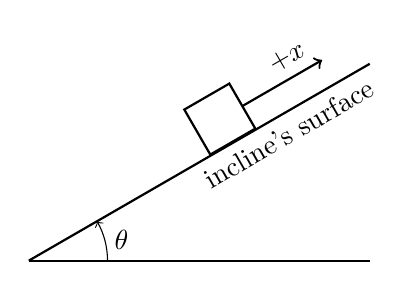
\begin{tikzpicture}
        %% Ramp
        \draw[thick] (0,0) -- (30:5cm)
            node[pos=1.00,anchor=north east,rotate=30] {incline's surface};
        \draw[thick] (0,0) -- (0:4.33cm);
        %% Angle
        \draw[->] (1.0,0) arc (0:30:1.0cm)
            node[pos=0.5,anchor=west] {$\theta$};
        %% Box
        \node[thick,draw,rectangle,minimum size=0.66cm,rotate=30,anchor=south]
            (B) at (30:3cm) {};
        %% Arrows
        \draw[thick,->] (B) -- ++ (30:1.5cm)
            node[pos=1.00,anchor=south east,rotate=30] {$+x$};
    \end{tikzpicture}
    \end{center}
    The mass remains at rest and the incline makes an angle $\theta$
        counterclockwise from the horizontal.
    Which one of the following choices best describes the
        orientation of the applied force by the person?
    The $+x$-axis is directed upward, parallel to the
        incline's surface as shown in the figure.
    \begin{choices}
        \wrongchoice{The applied force is oriented directly along the $+x$ axis.}
        \wrongchoice{The applied force is oriented at an angle $\theta$ clockwise from the $+x$ axis.}
      \correctchoice{The applied force is oriented at an angle $\ang{90}-\theta$ clockwise from the $+x$ axis.}
        \wrongchoice{The applied force is oriented at an angle $\ang{90}-\theta$ counterclockwise from the $+x$ axis.}
        \wrongchoice{This is a completely impossible situation that never can be realized physically.}
    \end{choices}
\end{question}
}

\element{aapt}{ %% Bowl-A3
\begin{question}{bowl-2015-q40}
    A \SI{2.0}{\kilo\gram} mass is connected to the end of string and moves about the string's fixed end in a conical motion with a constant speed of \SI{4.0}{\meter\per\second}.
    The string has a length of \SI{2.50}{\meter} and forms an angle of $\theta$ with the vertical.
    \begin{center}
    \begin{tikzpicture}
        %% Ceiling
        \node[anchor=south,fill,pattern=north east lines,minimum width=4cm, minimum height=0.05cm] at (0,0) {};
        \draw (-2,0) -- (2,0);
        %% Pendulum Bob
        \node[fill,draw,circle,minimum size=1em] (A) at (225:3cm) {};
        \draw (0,0) -- (A);
        %% Circular path
        \draw[dashed] (0,-2.21) circle (2.21cm and 0.5cm);
        %% Angle
        \draw[dashed] (0,0) -- (0,-2.21);
        \draw[<->] (225:1cm) arc (225:270:1cm) node[pos=0.5,anchor=north] {$\theta$};
    \end{tikzpicture}
    \end{center}
    What is the tension in the string?
    \begin{multicols}{2}
    \begin{choices}
        \wrongchoice{\SI{20.0}{\newton}}
        \wrongchoice{\SI{23.7}{\newton}}
      \correctchoice{\SI{27.4}{\newton}}
        \wrongchoice{\SI{29.8}{\newton}}
        \wrongchoice{\SI{32.5}{\newton}}
    \end{choices}
    \end{multicols}
\end{question}
}


%% PhysicsBowl 2014
%%----------------------------------------
\element{aapt}{ %% Bowl-A3
\begin{question}{bowl-2014-q04}
    Three equal masses are suspended from a classroom ceiling by a series of strings as shown in the figure.
    \begin{center}
    \begin{tikzpicture}[yscale=0.75]
        %% Ceiling
        \draw (-2,0) -- (2,0);
        \node[anchor=south,pattern=north east lines,minimum width=4cm,minimum height=0.05cm] at (0,0) {};
        %% Masses
        \node[draw,rectangle,anchor=center,minimum size=0.75cm] (A) at (0,-2) {$M$};
        \node[draw,rectangle,anchor=center,minimum size=0.75cm] (B) at (0,-4) {$M$};
        \node[draw,rectangle,anchor=center,minimum size=0.75cm] (C) at (0,-6) {$M$};
        %% Strings
        \draw[thick] (0,0) -- (A.north) node[pos=0.5,anchor=west] {$A$};
        \draw[thick] (A.south) -- (B.north) node[pos=0.5,anchor=west] {$B$};
        \draw[thick] (B.south) -- (C.north) node[pos=0.5,anchor=west] {$C$};
    \end{tikzpicture}
    \end{center}
    Which string has the greatest tension?
    \begin{choices}
      \correctchoice{Only String $A$.}
        \wrongchoice{Only String $B$.}
        \wrongchoice{Only String $C$.}
        \wrongchoice{Strings $A$, $B$, and $C$ have the same non-zero tension.}
        \wrongchoice{Strings $A$, $B$, and $C$ all have no tension.}
    \end{choices}
\end{question}
}

\element{aapt}{ %% Bowl-A3
\begin{question}{bowl-2014-q12}
    A box of mass \SI{5.0}{\kilo\gram} is being pushed to the right across a horizontal surface while a constant frictional force of \SI{8.0}{\newton} acts on the box.
    At some instant of time,
        the box has a speed of \SI{4.0}{\meter\per\second} and an acceleration of \SI{3.0}{\meter\per\second\squared}.
    What is the magnitude of the net force acting on the box at this instant?
    \begin{multicols}{3}
    \begin{choices}
        \wrongchoice{\SI{7.0}{\newton}}
        \wrongchoice{\SI{12.0}{\newton}}
      \correctchoice{\SI{15.0}{\newton}}
        \wrongchoice{\SI{20.0}{\newton}}
        \wrongchoice{\SI{23.0}{\newton}}
    \end{choices}
    \end{multicols}
\end{question}
}

\element{aapt}{ %% Bowl-A3
\begin{question}{bowl-2014-q14}
    A box rests on the floor of an elevator.
    The elevator is accelerating upward.
    Which one of the following choices best represents the Newton's Third Law pair force to the gravitational force acting on the box by the Earth?
    \begin{choices}
        \wrongchoice{There is no Newton's Third Law pair force in this scenario.}
        \wrongchoice{The entire normal force of contact from the floor on the box.}
        \wrongchoice{Only a portion of the normal force of contact from the floor on the box.}
        \wrongchoice{The force of the cables pulling upward on the elevator.}
      \correctchoice{The gravitational force acting on the Earth by the box.}
    \end{choices}
\end{question}
}

\element{aapt}{ %% Bowl-A3
\begin{question}{bowl-2014-q20}
    A uniform block of mass $m$ is placed on an inclined plane of angle $\theta$.
    \begin{center}
    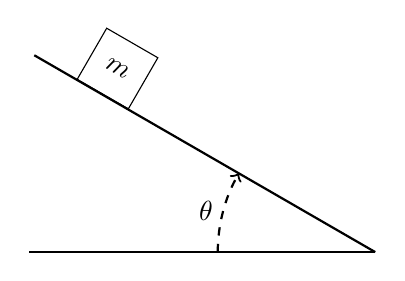
\begin{tikzpicture}
        %% Ramp
        \draw[thick] (0,0) -- ++ (150:5cm);
        \draw[thick] (0,0) -- ++ (180:4.4cm);
        %% Angle
        \draw[thick,->,dashed] (-2cm,0) arc (180:150:2cm) node[pos=0.5,anchor=east] {$\theta$};
        %% Box
        \node[draw,rotate=-30,minimum size=0.75cm,anchor=south] at (150:4cm) {$m$};
    \end{tikzpicture}
    \end{center}
    When released, the block does not move.
    It is determined that the normal force acting on the incline on the block has a magnitude of \SI{62}{\newton} while the force of static friction acting on the block has a magnitude of \SI{38}{\newton}.
    The coefficient of static friction between the block and inclined plane is $\mu_s = \num{0.92}$.
    Which one of the following choices best represents the mass, $m$, of the block?
    \begin{multicols}{3}
    \begin{choices}
        \wrongchoice{\SI{2.4}{\kilo\gram}}
        \wrongchoice{\SI{6.2}{\kilo\gram}}
      \correctchoice{\SI{7.3}{\kilo\gram}}
        \wrongchoice{\SI{8.4}{\kilo\gram}}
        \wrongchoice{\SI{10.0}{\kilo\gram}}
    \end{choices}
    \end{multicols}
\end{question}
}


%% PhysicsBowl 2013
%%----------------------------------------
\element{aapt}{ %% Bowl-A3
\begin{question}{bowl-2013-q16}
    A block initially moving at \SI{8.0}{\meter\per\second} accelerates uniformly to rest on a horizontal surface.
    The block travels a distance of \SI{12.0}{\meter} during the slide.
    Which one of the following choices best represents the coefficient of kinetic friction between the surface and the block?
    \begin{multicols}{3}
    \begin{choices}
        \wrongchoice{\num{1.20}}
        \wrongchoice{\num{0.667}}
        \wrongchoice{\num{0.533}}
      \correctchoice{\num{0.267}}
        \wrongchoice{\num{0.133}}
    \end{choices}
    \end{multicols}
\end{question}
}

\element{aapt}{ %% Bowl-A3
\begin{question}{bowl-2013-q28}
    An object is in free fall close to the ground.
    A person intervenes and slows the object uniformly to rest.
    Which one of the following statements must be true about the magnitude of the acceleration of the object as it is being stopped by the person?
    The magnitude of the object's acceleration is $a_{obj}$ and the magnitude of the acceleration from gravity is $g$.
    \begin{multicols}{2}
    \begin{choices}
        \wrongchoice{$a_{obj} = g$}
        \wrongchoice{$a_{obj} > g$}
        \wrongchoice{$a_{obj} < g$}
        \wrongchoice{$a_{obj} \leq g$}
        \wrongchoice{$a_{obj} \geq g$}
      \correctchoice{None of these relations must be true.}
    \end{choices}
    \end{multicols}
\end{question}
}


%% PhysicsBowl 2012
%%----------------------------------------
\element{aapt}{ %% Bowl-A3
\begin{question}{bowl-2012-q07}
    An object of mass \SI{5.00}{\kilo\gram} moves only to the right along the $+x$-axis.
    During some time interval, the object's speed increased from \SI{4.00}{\meter\per\second} to \SI{8.00}{\meter\per\second} with a constant acceleration of \SI{2.00}{\meter\per\second\squared}.
    What is the net force acting on the object during the time interval of the acceleration?
    \begin{multicols}{2}
    \begin{choices}
      \correctchoice{\SI{10.0}{\newton}}
        \wrongchoice{\SI{20.0}{\newton}}
        \wrongchoice{\SI{30.0}{\newton}}
        \wrongchoice{\SI{40.0}{\newton}}
        \wrongchoice{The answer cannot be determined without more information about the forces involved.}
    \end{choices}
    \end{multicols}
\end{question}
}

%% NOTE: bowl-2012-q10 -> Refer: bowl-2011-q10

\element{aapt}{ %% Bowl-A3
\begin{question}{bowl-2012-q10}
    A string of negligible mass connects an object of mass $M=\SI{10}{\kilo\gram}$ to the ceiling of an elevator.
    \begin{center}
    \begin{tikzpicture}[scale=1.33]
        \draw (0,0) rectangle (3,4);
        \node[anchor=north west] at (0,4) {elevator};
        \draw[thick] (1.5,4) -- ++(90:1);
        \node[minimum size=1cm,draw] (M) at (2,2) {$M$};
        \draw (M.north) -- (2.0,4) node[anchor=east,pos=0.33] {string};
    \end{tikzpicture}
    \end{center}
    The elevator experiences a constant downward acceleration of magnitude \SI{6.0}{\meter\per\second\squared}.
    Let $T$ represent the magnitude of the force by the string (tension) acting on the mass $M$,
        let $G$ represent the magnitude of the gravitational force by the Earth acting on the mass $M$,
        and let $F$ represent the magnitude of the net force acting on mass $M$.
    Which one of the following choices describes the relationship between these forces?
    \begin{multicols}{2}
    \begin{choices}
        \wrongchoice{$T=G=F$}
        \wrongchoice{$T<G<F$}
        \wrongchoice{$T=G<F$}
        \wrongchoice{$T<G=F$}
      \correctchoice{$T<G<F$}
    \end{choices}
    \end{multicols}
\end{question}
}

\element{aapt}{ %% Bowl-A3
\begin{question}{bowl-2012-q48}
    An object of mass $M$ is dropped from a height $H$
        above the ground.
    The object bounces off of a horizontal surface in a
        collision lasting time $T$.
    The object then rises upward to a maximum height
        $\frac{H}{2}$.
    What was the magnitude of the average net force
        acting on the mass during the collision
        with the surface?
    \begin{multicols}{2}
    \begin{choices}
        \wrongchoice{$\left(2-\sqrt{2}\right) \dfrac{M\sqrt{gH}}{T}$}
        \wrongchoice{$\left(\dfrac{1}{\sqrt{2}}+1\right) \dfrac{M\sqrt{gH}}{T}$}
        \wrongchoice{$\sqrt{3} \dfrac{M\sqrt{gH}}{T}$}
        \wrongchoice{$\left(2\sqrt{2}-1\right) \dfrac{M\sqrt{gH}}{T}$}
      \correctchoice{$\left(\sqrt{2}+1\right) \dfrac{M\sqrt{gH}}{T}$}
    \end{choices}
    \end{multicols}
\end{question}
}

%% PhysicsBowl 2011
%%----------------------------------------
\element{aapt}{ %% Bowl-A3
\begin{question}{bowl-2011-q06}
    A ball of mass $m=\SI{0.100}{\kilo\gram}$ is launched
        straight upward so that it rises to a maximum height
        of \SI{12.0}{\meter} above the launch point.
    Ignore air resistance.
    %% Start question
    When the ball reaches its maximum height, which one of the
        following choices best represents the magnitude of the
        net force acting on the ball?
    \begin{multicols}{3}
    \begin{choices}
        \wrongchoice{\SI{0}{\newton}}
        \wrongchoice{\SI{0.100}{\newton}}
      \correctchoice{\SI{1.00}{\newton}}
        \wrongchoice{\SI{10.0}{\newton}}
        \wrongchoice{\SI{12.0}{\newton}}
    \end{choices}
    \end{multicols}
\end{question}
}

\element{aapt}{ %% Bowl-A3
\begin{question}{bowl-2011-q10}
    A string of negligible mass connected an object of mass $M=\SI{10}{\kilo\gram}$ to the ceiling of an elevator.
    \begin{center}
    \begin{tikzpicture}[scale=1.33]
        \draw (0,0) rectangle (3,4);
        \node[anchor=north west] at (0,4) {elevator};
        \draw[thick] (1.5,4) -- ++(90:1);
        \node[minimum size=1cm,draw] (M) at (2,2) {$M$};
        \draw (M.north) -- (2.0,4) node[anchor=east,pos=0.33] {string};
    \end{tikzpicture}
    \end{center}
    The elevator experiences a constant downward speed of \SI{3.0}{\meter\per\second}.
    Let $T$ represent the magnitude of the force on the mass $M$ by the string (tension),
        $G$ represent the magnitude of the gravitational force by Earth acting on the mass $M$ hanging in the elevator, 
        and $F$ represent the magnitude of the net force acting on the mass $M$.
    Which one of the following choices describes the relationships between these forces?
    \begin{multicols}{2}
    \begin{choices}
        \wrongchoice{$F<T<G$}
        \wrongchoice{$F=T=G$}
        \wrongchoice{$F<G<T$}
        \wrongchoice{$F=T<G$}
      \correctchoice{$F<T=G$}
    \end{choices}
    \end{multicols}
\end{question}
}

\element{aapt}{ %% Bowl-A3
\begin{question}{bowl-2011-q12}
    A \SI{5.0}{\kilo\gram} mass moves along the $x$-axis.
    At one instant of time, the mass has position \SI{2.0}{\meter},
        velocity \SI{3.0}{\meter\per\second},
        and acceleration \SI{4.0}{\meter\per\second\squared}.
    What is the net force acting on the mass at this time?
    \begin{multicols}{3}
    \begin{choices}
        \wrongchoice{\SI{0}{\newton}}
        \wrongchoice{\SI{10.0}{\newton}}
        \wrongchoice{\SI{15.0}{\newton}}
      \correctchoice{\SI{20.0}{\newton}}
        \wrongchoice{\SI{22.5}{\newton}}
    \end{choices}
    \end{multicols}
\end{question}
}

\element{aapt}{ %% Bowl-A3
\begin{question}{bowl-2011-q13}
    A physics book sits at rest on a table.
    On top of the book is a calculator, also at rest.
    \begin{center}
    \begin{tikzpicture}
        %% table
        \node[anchor=south,draw,pattern=north east lines,minimum width=6cm,minimum height=2em] (T) at (0,0) {};
        \node[anchor=center,fill=white] at (0,1em) {Table};
        \fill (T.south west) ++(1em,0) rectangle ++(1em,-1);
        \fill (T.south east) ++(-1em,0) rectangle ++(-1em,-1);
        %% book
        \node[draw,fill=white!90!black,anchor=south,minimum width=3cm,minimum height=2em] (B) at (T.north) {Book};
        %% calculator
        \node[draw,anchor=south,minimum width=1cm,minimum height=1em,pin={40:Calculator}] (C) at (B.north) {};
    \end{tikzpicture}
    \end{center}
    Which one of the following choices is the Newton's Third Law pair force to the force that the table exerts on the book?
    \begin{choices}
      \correctchoice{The contact force on the table by the book.}
        \wrongchoice{The gravitational force on the book by the Earth.}
        \wrongchoice{The gravitational force on the combination of the book and calculator by the Earth.}
        \wrongchoice{The contact force on the book by the calculator.}
        \wrongchoice{The contact force on the table by the ground supporting it.}
    \end{choices}
\end{question}
}

\element{aapt}{ %% Bowl-A3
\begin{question}{bowl-2011-q15}
    A \SI{4.0}{\kilo\gram} object is pushed to the right on a rough surface by a horizontal force of \SI{15}{\newton} as shown.
    \begin{center}
    \begin{tikzpicture}
        %% floor
        \draw  (-3,0) -- (3,0);
        \node[anchor=north,pattern=north east lines,minimum width=6cm] at (0,0) {};
        %% Box
        \node[draw,minimum size=1.33cm,anchor=south] (A) at (-1,0) {\SI{4.0}{\kilo\gram}};
        \draw[thick,->] (A.east) -- ++(0:1.33) node[pos=0.5,anchor=south] {\SI{15}{\newton}};
    \end{tikzpicture}
    \end{center}
    During the push, the object accelerates uniformly to the right at \SI{2.50}{\meter\per\second}.
    What must be the magnitude of the force of friction also acting on the object during the push?
    %% NOTE: could rewrite and include direction
    \begin{multicols}{3}
    \begin{choices}
        \wrongchoice{\SI{0}{\newton}}
      \correctchoice{\SI{5}{\newton}}
        \wrongchoice{\SI{10}{\newton}}
        \wrongchoice{\SI{15}{\newton}}
        \wrongchoice{\SI{25}{\newton}}
    \end{choices}
    \end{multicols}
\end{question}
}

\element{aapt}{ %% Bowl-A3
\begin{question}{bowl-2011-q28}
    A person throws an object of mass $M$ straight upward with an initial non-zero speed $v$.
    The object rises to a maximum height $H$ above the launch point.
    The person now throws an object of mass $\frac{1}{2}M$ straight upward with speed $2v$.
    In terms of $H$, to what maximum height does the object of mass $\frac{1}{2}M$ rise above the launch point?
    Ignore air resistance?
    \begin{multicols}{3}
    \begin{choices}
        \wrongchoice{$8H$}
      \correctchoice{$4H$}
        \wrongchoice{$2H$}
        \wrongchoice{$\sqrt{2}H$}
        \wrongchoice{$H$}
    \end{choices}
    \end{multicols}
\end{question}
}

\element{aapt}{ %% Bowl-A3
\begin{question}{bowl-2011-q47}
    A simple pendulum of length $L$ has a point of mass $M$ released from rest from the horizontal position shown.
    In the absence of air resistance and friction,
        the mass swings through the arc of a circle.
    \begin{center}
    \begin{tikzpicture}
        \node[pin={120:pivot}] at (0,0) {};
        \draw (0,-0.25) -- (0.25,-0.25) -- (0.25,0);
        \draw[dashed] (3,0) arc (360:240:3);
        \node[anchor=south] at (1.5,0) {$L$};
        \draw[thick] (0,0) -- (3,0);
        \fill (3,0) circle (2pt) node[anchor=west] {$M$};
        \draw[thick] (0,0) -- (0,-3);
        \fill (0,-3) circle (2pt) node[anchor=north] {$P$};
    \end{tikzpicture}
    \end{center}
    Let $T$ represent the magnitude of the force from the string on the mass (tension),
        $G$ represent the magnitude of the gravitational force acting on the mass by the Earth,
        and $F$ represent the magnitude of the net force acting on the mass.
    Which one of the following choices describes the relationship among these forces when the mass swings at the bottom of the arc (point $P$)?
    \begin{multicols}{2}
    \begin{choices}
      \correctchoice{$G<F<T$}
        \wrongchoice{$F<G=T$}
        \wrongchoice{$F<G<T$}
        \wrongchoice{$T<F<G$}
        \wrongchoice{$G=F<T$}
    \end{choices}
    \end{multicols}
\end{question}
}


%% PhysicsBowl 2010
%%----------------------------------------
\element{aapt}{ %% Bowl-A3
\begin{question}{bowl-2010-q06}
    Which of the following statements is most closely associated
        with Newton's Third Law of Motion?
    \begin{choices}
        \wrongchoice{``What goes up must come down.''}
      \correctchoice{``For every action force, there is an equal but opposite reaction force.''}
        \wrongchoice{``An object at rest remains at rest.''}
        \wrongchoice{``The acceleration of an object is directly proportional to the force acting on the object but inversely proportional to the mass of the object.''}
        \wrongchoice{``The Universe tends toward disorder.''}
    \end{choices}
\end{question}
}

\element{aapt}{ %% Bowl-A3
\begin{question}{bowl-2010-q15}
    Three blocks, labeled $A$, $B$, and $C$, remain at rest on a table.
    \begin{center}
    \begin{tikzpicture}
        %% table
        \draw[pattern=north east lines] (-3,0) rectangle (3,-0.25);
        \draw[pattern=north east lines] (-2.75,-0.25) rectangle (-2.50,-1);
        \draw[pattern=north east lines] (+2.75,-0.25) rectangle (+2.50,-1);
        %% A, B, C
        \node[draw,fill=white!90!black,anchor=south,minimum width=5cm,minimum height=2em] (C) at (0,0) {\SI{13.0}{\newton}};
        \node[draw,fill=white!90!black,anchor=south,minimum width=4cm,minimum height=2em] (B) at (C.north) {\SI{7.0}{\newton}};
        \node[draw,fill=white!90!black,anchor=south,minimum width=3cm,minimum height=2em] (A) at (B.north) {\SI{5.0}{\newton}};
        %% labels
        \node[anchor=east] at (C.west) {$C$};
        \node[anchor=east] at (B.west) {$B$};
        \node[anchor=east] at (A.west) {$A$};
    \end{tikzpicture}
    \end{center}
    The magnitude of the gravitational force on each block is indicated on the figure.
    What is the magnitude of the contact force on block $C$ from block $B$?
    \begin{multicols}{3}
    \begin{choices}
        \wrongchoice{\SI{1.0}{\newton}}
        \wrongchoice{\SI{6.0}{\newton}}
        \wrongchoice{\SI{7.0}{\newton}}
      \correctchoice{\SI{12.0}{\newton}}
        \wrongchoice{\SI{13.0}{\newton}}
    \end{choices}
    \end{multicols}
\end{question}
}

\element{aapt}{ %% Bowl-A3
\begin{question}{bowl-2010-q32}
    A rubber ball of mass \SI{2.0}{\kilo\gram} falling straight
        downward hits the ground with a speed of
        \SI{0.90}{\meter\per\second} and then rebounds straight
        upward with a speed of \SI{0.60}{\meter\per\second}.
    The collision time of the ball with the ground is
        $t=\SI{0.25}{\second}$.
    Treat $g=\SI{20}{\meter\per\second\squared}$ for this
        situation.
    What is the magnitude of the average acceleration
        of the ball while it is in contact with the ground?
    \begin{multicols}{2}
    \begin{choices}
        \wrongchoice{\SI{1.2}{\meter\per\second\squared}}
      \correctchoice{\SI{6.0}{\meter\per\second\squared}}
        \wrongchoice{\SI{10.0}{\meter\per\second\squared}}
        \wrongchoice{\SI{13.0}{\meter\per\second\squared}}
        \wrongchoice{\SI{16.0}{\meter\per\second\squared}}
    \end{choices}
    \end{multicols}
\end{question}
}

\element{aapt}{ %% Bowl-A3
\begin{question}{bowl-2010-q33}
    A rubber ball of mass \SI{2.0}{\kilo\gram} falling straight
        downward hits the ground with a speed of
        \SI{0.90}{\meter\per\second} and then rebounds straight
        upward with a speed of \SI{0.60}{\meter\per\second}.
    The collision time of the ball with the ground is
        $t=\SI{0.25}{\second}$.
    Treat $g=\SI{20}{\meter\per\second\squared}$ for this
        situation.
    What is the magnitude of the average force
        exerted by the ground on the ball while they
        are in contact?
    \begin{multicols}{3}
    \begin{choices}
        \wrongchoice{\SI{2.4}{\newton}}
        \wrongchoice{\SI{12.0}{\newton}}
        \wrongchoice{\SI{20.0}{\newton}}
        \wrongchoice{\SI{26.0}{\newton}}
      \correctchoice{\SI{32.0}{\newton}}
    \end{choices}
    \end{multicols}
\end{question}
}


%% PhysicsBowl 2009
%%----------------------------------------
\element{aapt}{ %% Bowl-A3
\begin{question}{bowl-2009-q21}
    A \SI{20.0}{\kilo\gram} box remains at rest on a horizontal
        surface while a person pushes directly to the right
        on the box with a force of \SI{60}{\newton}.
    The coefficient of kinetic friction between the box and
        the surface is $\mu_k=\num{0.20}$.
    The coefficient of static friction between the box and
        the surface is $\mu_s=\num{0.60}$.
    What is the magnitude of the force of friction acting
        on the box during the push?
    \begin{multicols}{3}
    \begin{choices}
        \wrongchoice{\SI{200}{\newton}}
        \wrongchoice{\SI{120}{\newton}}
      \correctchoice{\SI{60}{\newton}}
        \wrongchoice{\SI{40}{\newton}}
        \wrongchoice{\SI{0}{\newton}}
    \end{choices}
    \end{multicols}
\end{question}
}


%% PhysicsBowl 2008
%%----------------------------------------
\element{aapt}{ %% Bowl-A3
\begin{question}{bowl-2008-q08}
    An object on an inclined plane has a gravitational force of magnitude \SI{10}{\newton} acting on it from the Earth.
    \begin{center}
    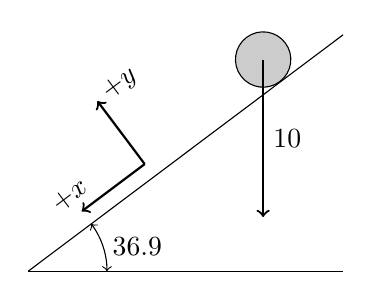
\begin{tikzpicture}
        %% Inclined Plan
        \draw (0,0) -- (36.9:5);
        \draw (0,0) -- (4,0);
        %% Object
        \node[draw,fill=white!80!black,circle,minimum size=2em,rotate=36.9,anchor=south] (M) at (36.9:4) {};
        \draw[thick,->] (M.center) -- ++(270:2) node[pos=0.5,anchor=west] {\SI{10}{\newton}};
        %% Angle
        \draw[<->] (1,0) arc (0:36.9:1) node[pos=0.5,anchor=west] {\ang{36.9}};
        %% Coordinates
        \draw[thick,->] (36.9:2) ++ (126.9:0.2) -- ++(126.9:1) node[anchor=west,rotate=36.9] {$+y$};
        \draw[thick,->] (36.9:2) ++ (126.9:0.2) -- ++(216.9:1) node[anchor=south,rotate=36.9] {$+x$};
    \end{tikzpicture}
    \end{center}
    Which of the following gives the correct components of this gravitational force for the coordinate axes shown in the figure?
    The $y$-axis is perpendicular to the incline's surface while the $x$-axis is parallel to the inclined surface.
    \begin{choices}
      \correctchoice{\makebox[6em][l]{$F_x = \SI{+6}{\newton}$,} \makebox[6em][l]{$F_y = \SI{-8}{\newton}$}}
        \wrongchoice{\makebox[6em][l]{$F_x = \SI{+8}{\newton}$,} \makebox[6em][l]{$F_y = \SI{-6}{\newton}$}}
        \wrongchoice{\makebox[6em][l]{$F_x = \SI{-6}{\newton}$,} \makebox[6em][l]{$F_y = \SI{+8}{\newton}$}}
        \wrongchoice{\makebox[6em][l]{$F_x = \SI{-8}{\newton}$,} \makebox[6em][l]{$F_y = \SI{+6}{\newton}$}}
        \wrongchoice{\makebox[6em][l]{$F_x = \SI{0}{\newton}$,}  \makebox[6em][l]{$F_y = \SI{10}{\newton}$}}
    \end{choices}
\end{question}
}

\element{aapt}{ %% Bowl-A3
\begin{question}{bowl-2008-q35}
    Astronauts on the Moon perform an experiment with a simple pendulum that is released from the horizontal position at rest.
    \begin{center}
    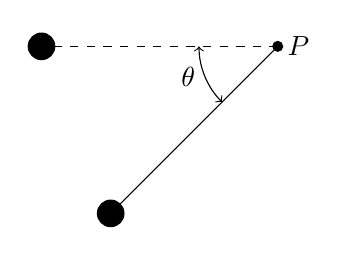
\begin{tikzpicture}
        %% point P
        \fill (0,0) circle (2pt) node[anchor=west] {$P$};
        %% initial position
        \draw[dashed] (0,0) -- (-3,0);
        \fill (-3,0) circle (5pt);
        %% theta position
        \draw (0,0) -- (225:3);
        \fill (225:3) circle (5pt);
        %% theta label
        \draw[<->] (-1,0) arc(180:225:1) node[pos=0.5,anchor=east] {$\theta$};
    \end{tikzpicture}
    \end{center}
    At the momentum shown in the diagram with $\ang{0}<\theta<\ang{90}$,
        the total acceleration of the mass may be directed in which of the following ways?
    \begin{choices}
      \correctchoice{straight to the right}
        \wrongchoice{straight to the left}
        \wrongchoice{straight upward}
        \wrongchoice{straight downward}
        \wrongchoice{straight along the connecting string toward point $P$ (the pivot)}
    \end{choices}
\end{question}
}


%% PhysicsBowl 2007
%%----------------------------------------
\element{aapt}{ %% Bowl-A3
\begin{question}{bowl-2007-q06}
    A \SI{500}{\kilo\gram} car is moving at \SI{28}{\meter\per\second}.
    The driver sees a barrier ahead.
    If the car takes \SI{95}{\meter} to come to rest,
        what is the magnitude of the minimum average force
        necessary to stop?
    \begin{multicols}{2}
    \begin{choices}
        \wrongchoice{\SI{47.5}{\newton}}
        \wrongchoice{\SI{1400}{\newton}}
      \correctchoice{\SI{2060}{\newton}}
        \wrongchoice{\SI{19 600}{\newton}}
        \wrongchoice{\SI{133 000}{\newton}}
    \end{choices}
    \end{multicols}
\end{question}
}

\element{aapt}{ %% Bowl-A3
\begin{question}{bowl-2007-q09}
    A block rests on an incline that makes the angle $\phi$ with the horizontal.
    The block remains at rest as $\phi$ is slowly increased.
    The magnitude of the normal force and the static frictional force of the incline on the block
    \begin{choices}
        \wrongchoice{both increase}
        \wrongchoice{both decrease}
        \wrongchoice{both remain the same}
        \wrongchoice{increase and decrease, respectively}
      \correctchoice{decrease and increase, respectively}
    \end{choices}
\end{question}
}

\element{aapt}{ %% Bowl-A3
\begin{question}{bowl-2007-q13}
    A student weighing \SI{500}{\newton} stands on a bathroom scale in the school's elevator.
    When the scale reads \SI{520}{\newton},
        the elevator must be:
    \begin{choices}
      \correctchoice{accelerating upward.}
        \wrongchoice{accelerating downward.}
        \wrongchoice{moving upward at a constant speed.}
        \wrongchoice{moving downward at a constant speed.}
        \wrongchoice{at rest.}
    \end{choices}
\end{question}
}

\element{aapt}{ %% Bowl-A3
\begin{question}{bowl-2007-q14}
    An object moves to the East across a frictionless surface with constant speed.
    A person then applies a constant force to the North on the object.
    What is the resulting path that the object takes?
    \begin{choices}
        \wrongchoice{A straight line path partly Eastward, partly Northward.}
        \wrongchoice{A straight line path totally to the North.}
      \correctchoice{A parabolic path opening toward the North.}
        \wrongchoice{A parabolic path opening toward the East.}
        \wrongchoice{An exponential path opening upward toward the North.}
    \end{choices}
\end{question}
}

\element{aapt}{ %% Bowl-A3
\begin{question}{bowl-2007-q18}
    In which one of the following situations is the net force constantly zero on the object?
    \begin{choices}
        \wrongchoice{A mass attached to a string and swinging like a pendulum.}
        \wrongchoice{A stone falling freely in a gravitational field.}
        \wrongchoice{An astronaut floating in the International Space Station.}
        \wrongchoice{A snowboarder riding down a steep hill.}
      \correctchoice{A skydiver who has reached terminal velocity.}
    \end{choices}
\end{question}
}

\element{aapt}{ %% Bowl-A3
\begin{question}{bowl-2007-q19}
    What net force is necessary to keep a \SI{1.0}{\kilo\gram} puck moving in a circle of radius \SI{0.5}{\meter} on a horizontal frictionless surface with a speed of \SI{2.0}{\meter\per\second}?
    \begin{multicols}{3}
    \begin{choices}
        \wrongchoice{\SI{0}{\newton}}
        \wrongchoice{\SI{2.0}{\newton}}
        \wrongchoice{\SI{4.0}{\newton}}
      \correctchoice{\SI{8.0}{\newton}}
        \wrongchoice{\SI{16}{\newton}}
    \end{choices}
    \end{multicols}
\end{question}
}

\element{aapt}{ %% Bowl-A3
\begin{question}{bowl-2007-q20}
    A large wedge rests on a horizontal frictionless surface,
        as shown.
    \begin{center}
    \begin{tikzpicture}
        %% Floor
        \draw (-1,0) -- (5,0);
        \node[anchor=north,pattern=north east lines,minimum width=6cm] at (2,0) {};
        %% Wedge
        \draw[fill=white!90!black] (0,0) -- (4,3) -- (4,0) -- cycle;
        %% block
        \node[anchor=south,draw,fill=white!60!black,minimum size=1cm,rotate=36.8] at (36.8:3) {};
    \end{tikzpicture}
    \end{center}
    A block starts from rest and slides down the inclined surface of the wedge,
        which is rough.
    During the motion of the block,
        the center of mass of the block and wedge system.
    \begin{choices}
        \wrongchoice{does not move.}
      \correctchoice{moves vertically with increasing speed.}
        \wrongchoice{moves horizontally with constant speed.}
        \wrongchoice{moves horizontally with increasing speed.}
        \wrongchoice{moves both horizontally and vertically.}
    \end{choices}
\end{question}
}

\element{aapt}{ %% Bowl-A3
\begin{question}{bowl-2007-q21}
    A box slides to the right across a horizontal floor.
    A person called Ted exerts a force $T$ to the right on the box.
    A person called Mario exerts a force $M$ to the left,
        which is half as large as the force $T$.
    Given that there is friction $f$ and the box accelerates to the right,
        rank the sizes of these three forces exerted on the box.
    \begin{multicols}{2}
    \begin{choices}
      \correctchoice{$f<M<T$}
        \wrongchoice{$M<f<T$}
        \wrongchoice{$M<T<f$}
        \wrongchoice{$f=M<T$}
        \wrongchoice{It cannot be determined.}
    \end{choices}
    \end{multicols}
\end{question}
}


%% PhysicsBowl 2006
%%----------------------------------------
\element{aapt}{ %% Bowl-A3
\begin{question}{bowl-2006-q05}
    Newton's First Law is based on the experimental work of which person,
        who rolled spheres down and up inclines?
    \begin{multicols}{2}
    \begin{choices}
      \correctchoice{Galileo Galilei}
        \wrongchoice{Christian Huygens}
        \wrongchoice{Nicolas Copernicus}
        \wrongchoice{Count Rumford}
        \wrongchoice{Aristotle}
    \end{choices}
    \end{multicols}
\end{question}
}

\element{aapt}{ %% Bowl-A3
\begin{question}{bowl-2006-q08}
    A baseball is thrown by a pitcher with a speed of \SI{35}{\meter\per\second}.
    The batter swings and hits the ball.
    The magnitude of the force that the ball exerts on the bat is always:
    \begin{choices}
        \wrongchoice{zero as it is only the bat that exerts a force on the ball.}
        \wrongchoice{equal to the gravitational force acting on the ball.}
        \wrongchoice{larger than the force the bat exerts on the ball.}
        \wrongchoice{smaller than the force the bat exerts on the ball.}
      \correctchoice{equal to the force that the bat exerts on the ball.}
    \end{choices}
\end{question}
}

\element{aapt}{ %% Bowl-A3
\begin{question}{bowl-2006-q15}
    A crate of toys remains at rest on a sleigh as the sleigh is pulled
        up a hill with an increasing speed.
    The crate is not fastened down to the sleigh.
    What force is responsible for the crate's increase in speed up the hill?
    \begin{choices}
        \wrongchoice{the contact force (normal force) of the ground on the sleigh}
      \correctchoice{the force of static friction of the sleigh on the crate}
        \wrongchoice{the contact force (normal force) of the sleigh on the crate}
        \wrongchoice{the gravitational force acting on the sleigh}
        \wrongchoice{no force is needed}
    \end{choices}
\end{question}
}


%% PhysicsBowl 2005
%%----------------------------------------
\element{aapt}{ %% Bowl-A3
\begin{question}{bowl-2005-q03}
    What is the centripetal acceleration of an object (mass = \SI{50}{\gram}) on the end of an \SI{80}{\centi\meter} string rotating at a constant rate of 4 times a second?
    \begin{center}
    \begin{tikzpicture}
        \draw[dashed] (0,0) circle (2);
        \draw[fill] (40:2) circle (3pt) node[anchor=west,xshift=3pt] {\SI{50}{\gram}};
        \draw[thick,->] (40:2) arc(40:60:2);
        \draw (0,0) -- (40:2) node[pos=0.5,anchor=south,rotate=40] {\SI{80}{\centi\meter}};
    \end{tikzpicture}
    \end{center}
    \begin{multicols}{2}
    \begin{choices}
        \wrongchoice{\SI{25}{\meter\per\second\squared}}
        \wrongchoice{\SI{32}{\meter\per\second\squared}}
        \wrongchoice{\SI{100}{\meter\per\second\squared}}
      \correctchoice{\SI{500}{\meter\per\second\squared}}
        \wrongchoice{\SI{2500}{\meter\per\second\squared}}
    \end{choices}
    \end{multicols}
\end{question}
}

\element{aapt}{ %% Bowl-A3
\begin{question}{bowl-2005-q06}
    The students in a Physics I class were in lab conducting an experiment related to Newton's Second Law.
    The collected data were displayed on the graph below.
    \begin{center}
    %% Changed net force to force
    \begin{tikzpicture}
        \begin{axis}[
            axis y line=left,
            axis x line=bottom,
            axis line style={->},
            xlabel={acceleration},
            x unit=\si{\meter\per\second\squared},
            xtick={0,0.2,0.4,0.6,0.8,1.0},
            ylabel={force},
            y unit=\si{\newton},
            ytick={0,5,10,15,20,25},
            grid=major,
            xmin=0,xmax=1.05,
            ymin=0,ymax=26,
            width=0.8\columnwidth,
            height=0.5\columnwidth,
        ]
        \addplot[line width=1pt,mark=*] plot coordinates {(0,0) (10,23)};
        \end{axis}
    \end{tikzpicture}
    \end{center}
    From this graph, what conclusions can the students make?
    \begin{choices}
      \correctchoice{The mass of the system was constant.}
        \wrongchoice{The acceleration of the system was constant.}
        \wrongchoice{The force acting on the system}
        \wrongchoice{The force acting on the system is not related to the acceleration of the system.}
        \wrongchoice{The force acting on any system will always be less than 20 N.}
    \end{choices}
\end{question}
}

\element{aapt}{ %% Bowl-A3
\begin{question}{bowl-2005-q08}
    Why do raindrops fall with constant speed during the later stages of their descent?
    \begin{choices}
        \wrongchoice{The gravitational force is the same for all drops.}
        \wrongchoice{All drops fall from the same height.}
        \wrongchoice{The gravitational force is negligible for objects as small as raindrops.}
        \wrongchoice{The gravitational force cannot increase the speed of a falling object to more than 9.8 m/s.}
      \correctchoice{Air resistance balances the gravitational force on a drop.}
    \end{choices}
\end{question}
}

\element{aapt}{ %% Bowl-A3
\begin{question}{bowl-2005-q13}
    A bat striking a \SI{0.125}{\kilo\gram} baseball is in contact
        with the ball for a time of \SI{0.03}{\second}.
    The ball travels in a straight line as it approaches and then leaves the bat.
    If the ball arrives at the bat with a velocity of
        \SI{4.5}{\meter\per\second} and leaves with a velocity of \SI{-6.5}{\meter\per\second},
        what is the magnitude of the average force acting on the ball?
    \begin{multicols}{2}
    \begin{choices}
        \wrongchoice{\SI{8.33}{\newton}}
        \wrongchoice{\SI{18.75}{\newton}}
        \wrongchoice{\SI{27.08}{\newton}}
      \correctchoice{\SI{45.83}{\newton}}
        \wrongchoice{\SI{458}{\newton}}
    \end{choices}
    \end{multicols}
\end{question}
}

\element{aapt}{ %% Bowl-A3
\begin{question}{bowl-2005-q14}
    An astronaut on the Moon simultaneously drops a feather and a hammer.
    The fact that they reach the surface at the same instant shows that
    \begin{choices}
        \wrongchoice{no gravity forces act on a body in a vacuum.}
        \wrongchoice{the acceleration due to gravity on the Moon is less than the acceleration due to gravity on the Earth.}
        \wrongchoice{the gravitational force from the Moon on heavier objects (the hammer) is equal to the gravitational force on lighter objects (the feather).}
        \wrongchoice{a hammer and feather have less mass on the Moon than on Earth.}
      \correctchoice{in the absence of air resistance all bodies at a given location fall with the same acceleration.}
    \end{choices}
\end{question}
}


%% PhysicsBowl 2000
%%----------------------------------------
\element{aapt}{ %% Bowl-A3
\begin{question}{bowl-2000-q13}
    An object near the surface of the earth with a weight of
        \SI{100}{\newton} is accelerated at \SI{4}{\meter\per\second\squared}.
    What is the net force on the object?
    \begin{multicols}{2}
    \begin{choices}
        \wrongchoice{\SI{25}{\newton}}
      \correctchoice{\SI{40}{\newton}}
        \wrongchoice{\SI{250}{\newton}}
        \wrongchoice{\SI{400}{\newton}}
        \wrongchoice{\SI{2500}{\newton}}
    \end{choices}
    \end{multicols}
\end{question}
}

\element{aapt}{ %% Bowl-A3
\begin{question}{bowl-2000-q21}
    %The next TWO questions will refer to the following information.
    A car of mass $m$ slides across a patch of ice at a speed $v$ with its brakes locked.
    It then hits dry pavement and skids to a stop in a distance $d$.
    The coefficient of kinetic friction between the tires and the dry road is $\mu$.
    %% Start Question
    If the car had a mass of $2m$, it would have skidded a distance of:
    \begin{multicols}{3}
    \begin{choices}
        \wrongchoice{$\dfrac{1}{2} d$}
      \correctchoice{$d$}
        \wrongchoice{$\sqrt{2} d$}
        \wrongchoice{$2 d$}
        \wrongchoice{$4 d$}
        %% NOTE: Added for symmetry
        \wrongchoice{$\dfrac{1}{4} d$}
    \end{choices}
    \end{multicols}
\end{question}
}

\element{aapt}{ %% Bowl-A3
\begin{question}{bowl-2000-q22}
    %The next TWO questions will refer to the following information.
    A car of mass $m$ slides across a patch of ice at a speed $v$ with its brakes locked.
    It then hits dry pavement and skids to a stop in a distance $d$.
    The coefficient of kinetic friction between the tires and the dry road is $\mu$.
    %% Start Question
    If the car had a speed of $2v$, it would have skidded a distance of:
    \begin{multicols}{3}
    \begin{choices}
        \wrongchoice{$\dfrac{1}{2} d$}
        \wrongchoice{$d$}
        \wrongchoice{$\sqrt{2} d$}
        \wrongchoice{$2 d$}
      \correctchoice{$4 d$}
        %% NOTE: Added for symmetry
        \wrongchoice{$\dfrac{1}{4} d$}
    \end{choices}
    \end{multicols}
\end{question}
}

\element{aapt}{ %% Bowl-A3
\begin{question}{bowl-2000-q25}
    The net force on a rocket with a weight of \SI{1.5e4}{\newton} is \SI{2.4e4}{\newton}.
    About how much time is needed to increase the rocket's speed
        from \SI{12}{\meter\per\second} to \SI{36}{\meter\per\second}
        near the surface of the Earth at takeoff?
    \begin{multicols}{3}
    \begin{choices}
        \wrongchoice{\SI{0.62}{\second}}
        \wrongchoice{\SI{0.78}{\second}}
      \correctchoice{\SI{1.5}{\second}}
        \wrongchoice{\SI{3.8}{\second}}
        \wrongchoice{\SI{15}{\second}}
    \end{choices}
    \end{multicols}
\end{question}
}

\element{aapt}{ %% Bowl-A3
\begin{question}{bowl-2000-q26}
    A \SI{500}{\gram} ball moving at \SI{15}{\meter\per\second}
        slows down uniformly until it stops.
    If the ball travels \SI{15}{\meter},
        what was the average net force applied while it was coming to a stop?
    \begin{multicols}{2}
    \begin{choices}
        \wrongchoice{\SI{0.37}{\newton}}
      \correctchoice{\SI{3.75}{\newton}}
        \wrongchoice{\SI{37.5}{\newton}}
        \wrongchoice{\SI{375}{\newton}}
        \wrongchoice{\SI{3750}{\newton}}
    \end{choices}
    \end{multicols}
\end{question}
}

\element{aapt}{ %% Bowl-A3
\begin{question}{bowl-2000-q32}
    A block rests on a flat plane inclined at an angle of \ang{30} with respect to the horizontal.
    What is the minimum coefficient of friction necessary to keep the block from sliding?
    \begin{multicols}{3}
    \begin{choices}
        \wrongchoice{$\dfrac{1}{2}$}
        \wrongchoice{$\dfrac{1}{\sqrt{2}}$}
      \correctchoice{$\dfrac{1}{\sqrt{3}}$}
        \wrongchoice{$\dfrac{1}{4}$}
        \wrongchoice{$\dfrac{2}{\sqrt{3}}$}
    \end{choices}
    \end{multicols}
\end{question}
}


%% PhysicsBowl 1999
%%----------------------------------------
\element{aapt}{ %% Bowl-A3
\begin{question}{bowl-1999-q02}
    Which of the following terms is \emph{not} related
        conceptually to the others?
    \begin{multicols}{2}
    \begin{choices}
        \wrongchoice{vector}
        \wrongchoice{resultant}
        \wrongchoice{component}
      \correctchoice{exponent}
        \wrongchoice{equilibrant}
    \end{choices}
    \end{multicols}
\end{question}
}

\element{aapt}{ %% Bowl-A3
\begin{question}{bowl-1999-q03}
    If the net force on an object were doubled while
        at the same time the mass of the object was
        halved, then the acceleration of the object is:
    \begin{multicols}{2}
    \begin{choices}
        \wrongchoice{\num{1/4} as great}
        \wrongchoice{\num{1/2} as great}
        \wrongchoice{\num{2} times as great}
      \correctchoice{\num{4} times as great}
        \wrongchoice{unchanged}
    \end{choices}
    \end{multicols}
\end{question}
}

\element{aapt}{ %% Bowl-A3
\begin{question}{bowl-1999-q05}
    A tractor-trailer truck is traveling down the road.
    The mass of the trailer is \num{4} times the mass
        of the tractor.
    If the tractor accelerates forward, the force
        that the trailer applies on the tractor is
    \begin{choices}
        \wrongchoice{\num{4} times greater than the force of the tractor on the trailer.}
        \wrongchoice{\num{2} times greater than the force of the tractor on the trailer.}
      \correctchoice{equal to the force of the tractor on the trailer.}
        \wrongchoice{\num{1/4} the force of the tractor on the trailer.}
        \wrongchoice{zero since the tractor is pulling the trailer forward.}
    \end{choices}
\end{question}
}

\element{aapt}{ %% Bowl-A3
\begin{question}{bowl-1999-q12}
    Two boxes are accelerated to the right on a frictionless horizontal surface as shown.
    \begin{center}
    \begin{tikzpicture}
        %% Floor
        \node[anchor=north,fill,pattern=north east lines,minimum width=7cm, minimum height=0.05cm] at (0,0) {};
        \draw (-3.5,0) -- (3.5,0);
        %% Masses
        \node[draw,fill=white!80!black,rectangle,rounded corners=1ex,minimum size=1.00cm,anchor=south east] (A) at (-2,0) {\SI{3}{\kilo\gram}};
        \node[draw,fill=white!80!black,rectangle,rounded corners=1ex,minimum size=1.43cm,anchor=south west] (B) at (+0,0) {\SI{9}{\kilo\gram}};
        %% string
        \draw[thick] (A.south east) ++ (90:0.66) -- ++(0:2) node[pos=0.5,anchor=south] {};
        \draw[thick,->] (B.east) -- ++(0:1.5) node[pos=0.5,anchor=south] {\SI{24}{\newton}};
    \end{tikzpicture}
    \end{center}
    The larger box has a mass of \SI{9}{\kilo\gram} and the smaller box has a mass of \SI{3}{\kilo\gram}.
    If a \SI{24}{\newton} horizontal force pulls on the larger box,
        with what force does the larger box pull the smaller box?
    \begin{multicols}{3}
    \begin{choices}
        \wrongchoice{\SI{3}{\newton}}
      \correctchoice{\SI{6}{\newton}}
        \wrongchoice{\SI{8}{\newton}}
        \wrongchoice{\SI{18}{\newton}}
        \wrongchoice{\SI{24}{\newton}}
    \end{choices}
    \end{multicols}
\end{question}
}

\element{aapt}{ %% Bowl-A3
\begin{question}{bowl-1999-q16}
    Which of the following principles best explains why
        large tractor-trailer trucks generally accelerate
        much more slowly than automobiles?
    \begin{choices}
        %% NOTE: Newton's second law
        \wrongchoice{To every action there is an equal reaction.}
        \wrongchoice{Every body attracts every other body in the universe.}
        \wrongchoice{A force is necessary to change the speed or direction of a body.}
        \wrongchoice{The total momentum of interacting bodies is always conserved.}
      \correctchoice{The acceleration of a body is inversely proportional to its
            mass and directly proportional to the external force acting on the body.}
    \end{choices}
\end{question}
}

\element{aapt}{ %% Bowl
\begin{question}{bowl-1999-q36}
    What happens to the inertia at an object when its velocity is doubled?
    \begin{choices}
        \wrongchoice{the object's inertia becomes $\sqrt{2}$ times greater}
        \wrongchoice{the object's inertia becomes \num{2} times greater}
        \wrongchoice{the object's inertia becomes \num{4} times greater}
        \wrongchoice{the object's inertia becomes \num{8} times greater}
      \correctchoice{the object's inertia is unchanged}
    \end{choices}
\end{question}
}

\element{aapt}{ %% Bowl-A3
\begin{questionmult}{bowl-1999-q39}
    The driver of an automobile must carefully control each of the following devices.
    Which of these devices can cause an acceleration in a moving car?
    \begin{choices}
      \correctchoice{the break pedal}
      \correctchoice{the gas pedal}
      \correctchoice{the steering wheel}
    \end{choices}
\end{questionmult}
}



%% PhysicsBowl 1998
%%----------------------------------------
\element{aapt}{ %% Bowl-A3
\begin{question}{bowl-1998-q03}
    An object in equilibrium has three forces, $F_1=\SI{30}{\newton}$,
        $F_2=\SI{50}{\newton}$, and $F_3=\SI{70}{\newton}$, acting on it.
    The magnitude of the resultant of $F_1$ and $F_2$ is:
    \begin{multicols}{3}
    \begin{choices}
        \wrongchoice{\SI{10}{\newton}}
        \wrongchoice{\SI{20}{\newton}}
        \wrongchoice{\SI{40}{\newton}}
      \correctchoice{\SI{70}{\newton}}
        \wrongchoice{\SI{80}{\newton}}
        %% NOTE: zero is a good distractor
        \wrongchoice{\SI{0}{\newton}}
    \end{choices}
    \end{multicols}
\end{question}
}

\element{aapt}{ %% Bowl-A3
\begin{question}{bowl-1998-q16}
    If the unit for force is $\mathrm{F}$, the unit for velocity $\mathrm{V}$,
        and the unit for time $\mathrm{T}$, then the unit for momentum is:
    \begin{multicols}{3}
    \begin{choices}
      \correctchoice{$\mathrm{FT}$}
        \wrongchoice{$\mathrm{FTV}$}
        \wrongchoice{$\mathrm{FT}^2V$}
        \wrongchoice{$\dfrac{\mathrm{FT}}{\mathrm{V}}$}
        \wrongchoice{$\dfrac{\mathrm{FV}}{\mathrm{T}}$}
    \end{choices}
    \end{multicols}
\end{question}
}

\element{aapt}{ %% Bowl-A3
\begin{question}{bowl-1998-q25}
    A car whose mass is \SI{1200}{\kilo\gram} is accelerated from rest by a constant force of \SI{2 400}{\newton}.
    What is the speed of the car \SI{8.0}{\second} after beginning?
    \begin{multicols}{3}
    \begin{choices}
        \wrongchoice{\SI{0.40}{\meter\per\second}}
        \wrongchoice{\SI{1.6}{\meter\per\second}}
        \wrongchoice{\SI{4.0}{\meter\per\second}}
        \wrongchoice{\SI{8.0}{\meter\per\second}}
      \correctchoice{\SI{16}{\meter\per\second}}
    \end{choices}
    \end{multicols}
\end{question}
}

\element{aapt}{ %% Bowl-A3
\begin{question}{bowl-1998-q29}
    A \SI{50}{\kilo\gram} student stands on a scale in an elevator.
    At the instant the elevator has a downward acceleration of \SI{1.0}{\meter\per\second\squared} and an upward velocity of \SI{3.0}{\meter\per\second},
        the scale reads approximately:
    \begin{multicols}{3}
    \begin{choices}
        \wrongchoice{\SI{350}{\newton}}
      \correctchoice{\SI{450}{\newton}}
        \wrongchoice{\SI{500}{\newton}}
        \wrongchoice{\SI{550}{\newton}}
        \wrongchoice{\SI{650}{\newton}}
    \end{choices}
    \end{multicols}
\end{question}
}

\element{aapt}{ %% Bowl-A3
\begin{question}{bowl-1998-q32}
    A \SI{3.0}{\kilo\gram} block with initial speed \SI{4.0}{\meter\per\second} slides across a rough horizontal floor before coming to rest.
    The frictional force acting on the block is \SI{3.0}{\newton}.
    How far does the block slide before coming to rest?
    \begin{multicols}{3}
    \begin{choices}
        \wrongchoice{\SI{1.0}{\meter}}
        \wrongchoice{\SI{2.0}{\meter}}
        \wrongchoice{\SI{4.0}{\meter}}
      \correctchoice{\SI{8.0}{\meter}}
        \wrongchoice{\SI{16}{\meter}}
    \end{choices}
    \end{multicols}
\end{question}
}


%% PhysicsBowl 1997
%%----------------------------------------
\element{aapt}{ %% Bowl-A3
\begin{question}{bowl-1997-q08}
    Cart 1 and cart 2 are held together as shown in the diagram below.
    Cart 2 is more massive than cart 1.
    \begin{center}
    \begin{tikzpicture}
        %% floor
        \draw (-3,0) -- (3,0);
        \node[anchor=north,pattern=north east lines,minimum width=6cm] at (0,0) {};
        %% cart 1
        \node[anchor=south,draw,minimum width=1.66cm,minimum height=0.5cm] (A) at (-1.66,1em) {1};
        \draw (A.south west) ++(+0.5em,-0.5em) circle (0.5em);
        \draw (A.south east) ++(-0.5em,-0.5em) circle (0.5em);
        %% cart 2
        \node[anchor=south,draw,minimum width=1.66cm,minimum height=1.0cm] (B) at (+1.66,1em) {2};
        \draw (B.south west) ++(+0.5em,-0.5em) circle (0.5em);
        \draw (B.south east) ++(-0.5em,-0.5em) circle (0.5em);
        %% String
        \draw[decoration={aspect=0.2,segment length=1.5mm,amplitude=1.5mm,coil},decorate] (A.east) -- ++(0:1.66cm);
    \end{tikzpicture}
    \end{center}
    As they are forced apart by the release of a compressed spring,
        which of the following quantities will have the same magnitude for both carts?
    \begin{multicols}{2}
    \begin{choices}
        \wrongchoice{acceleration}
        \wrongchoice{change of velocity}
      \correctchoice{force}
        \wrongchoice{speed}
        \wrongchoice{velocity}
    \end{choices}
    \end{multicols}
\end{question}
}

\element{aapt}{ %% Bowl-A3
\begin{question}{bowl-1997-q30}
    A string with masses of \SI{1.5}{\kilo\gram} and \SI{3.0}{\kilo\gram} on its ends is hung over a frictionless,
        massless pulley as shown below.
    \begin{center}
    \begin{tikzpicture}
        %% Ceiling
        \node[anchor=south,fill,pattern=north east lines,minimum width=4cm, minimum height=0.05cm] at (0,0) {};
        \draw (-2,0) -- (2,0);
        %% Pulley
        \draw (0,-1) circle (0.75);
        \draw[fill=white!90!black] (-0.3,0) -- (-0.2,-1.1) arc(190:350:0.2) -- (0.3,0) --cycle;
        \draw[fill] (0,-1) circle (1.5pt);
        %% Masses
        \node[draw,fill=white!90!black,rectangle,rounded corners=1ex,minimum size=1cm,anchor=north] (A) at (-0.75,-4) {\SI{1.5}{\kilo\gram}};
        \node[draw,fill=white!90!black,rectangle,rounded corners=1ex,minimum size=1.414cm,anchor=north] (B) at (0.75,-3) {\SI{3.0}{\kilo\gram}};
        %% Rope
        \draw[thick] (A.north) -- (-0.75,-1.0) arc(180:0:0.75) -- (B.north);
    \end{tikzpicture}
    \end{center}
    What is the approximate magnitude of the acceleration of the masses?
    \begin{multicols}{2}
    \begin{choices}
        \wrongchoice{\SI{1.5}{\meter\per\second\squared}}
        \wrongchoice{\SI{3.0}{\meter\per\second\squared}}
      \correctchoice{\SI{3.3}{\meter\per\second\squared}}
        \wrongchoice{\SI{6.7}{\meter\per\second\squared}}
        \wrongchoice{\SI{10}{\meter\per\second\squared}}
    \end{choices}
    \end{multicols}
\end{question}
}

\element{aapt}{ %% Bowl-A3
\begin{question}{bowl-1997-q31}
    Two blocks of mass \SI{1.0}{\kilo\gram} and \SI{3.0}{\kilo\gram} are connected by a string which has a tension of \SI{2.0}{\newton}.
    A force $F$ acts on the \SI{3.0}{\kilo\gram} block as shown below.
    %% NOTE: bowl-1999-q12
    \begin{center}
    \begin{tikzpicture}
        %% Floor
        \node[anchor=north,fill,pattern=north east lines,minimum width=7cm, minimum height=0.05cm] at (0,0) {};
        \draw (-3.5,0) -- (3.5,0);
        %% Masses
        \node[draw,fill=white!80!black,rectangle,rounded corners=1ex,minimum size=1.00cm,anchor=south east] (A) at (-2,0) {\SI{1}{\kilo\gram}};
        \node[draw,fill=white!80!black,rectangle,rounded corners=1ex,minimum size=1.43cm,anchor=south west] (B) at (+0,0) {\SI{3}{\kilo\gram}};
        %% string
        \draw[thick] (A.south east) ++ (90:0.66) -- ++(0:2cm) node[pos=0.5,anchor=south] {\SI{2}{\newton}};
        \draw[thick,->] (B.east) -- ++(0:1.5) node[pos=0.5,anchor=south] {$F$};
    \end{tikzpicture}
    \end{center}
    Assuming friction is negligible, what is the value of $F$?
    \begin{multicols}{3}
    \begin{choices}
        \wrongchoice{\SI{1.0}{\newton}}
        \wrongchoice{\SI{2.0}{\newton}}
        \wrongchoice{\SI{4.0}{\newton}}
        \wrongchoice{\SI{6.0}{\newton}}
      \correctchoice{\SI{8.0}{\newton}}
    \end{choices}
    \end{multicols}
\end{question}
}

\element{aapt}{ %% Bowl-A3
\begin{question}{bowl-1997-q33}
    A softball player catches a ball of mass $m$,
        which is moving toward her with horizontal speed $v$.
    While bringing the ball to rest,
        her hand moves back a distance $d$.
    Assuming constant deceleration,
        the horizontal force exerted on the ball by her hand is:
    \begin{multicols}{3}
    \begin{choices}
      \correctchoice{$\dfrac{mv^2}{2d}$}
        \wrongchoice{$\dfrac{mv^2}{d}$}
        \wrongchoice{$mvd$}
        \wrongchoice{$\dfrac{2mv}{d}$}
        \wrongchoice{$\dfrac{mv}{d}$}
    \end{choices}
    \end{multicols}
\end{question}
}


%% PhysicsBowl 1996
%%----------------------------------------
\element{aapt}{ %% Bowl-A3
\begin{question}{bowl-1996-q09}
    When a falling object reaches terminal velocity, it:
    \begin{choices}
        \wrongchoice{is no longer subject to the friction of air.}
      \correctchoice{moves downward with constant velocity.}
        \wrongchoice{has an acceleration of approximately \SI{10}{\meter\per\second\squared}.}
        \wrongchoice{has no downward velocity.}
        \wrongchoice{has an upward acceleration.}
    \end{choices}
\end{question}
}

\element{aapt}{ %% Bowl-A3
\begin{question}{bowl-1996-q15}
    A car whose mass is \SI{1500}{\kilo\gram} is accelerated uniformly from rest to a speed of \SI{20}{\meter\per\second} in \SI{10}{\second}.
    The magnitude of the net force accelerating the car is:
    \begin{multicols}{2}
    \begin{choices}
        \wrongchoice{\SI{1 000}{\newton}}
        \wrongchoice{\SI{2 000}{\newton}}
      \correctchoice{\SI{3 000}{\newton}}
        \wrongchoice{\SI{20 000}{\newton}}
        \wrongchoice{\SI{30 000}{\newton}}
    \end{choices}
    \end{multicols}
\end{question}
}

\element{aapt}{ %% Bowl-A3
\begin{question}{bowl-1996-q30}
    An \SI{800}{\kilo\gram} elevator accelerates downward at \SI{2.0}{\meter\per\second\squared}.
    The force exerted by the cable on the elevator is:
    \begin{multicols}{2}
    \begin{choices}
        \wrongchoice{\SI{1.6}{\kilo\newton} down}
        \wrongchoice{\SI{1.6}{\kilo\newton} up}
      \correctchoice{\SI{6.4}{\kilo\newton} up}
        \wrongchoice{\SI{8.0}{\kilo\newton} down}
        \wrongchoice{\SI{9.6}{\kilo\newton} down}
    \end{choices}
    \end{multicols}
\end{question}
}

\element{aapt}{ %% Bowl-A3
\begin{question}{bowl-1996-q32}
    The \SI{10.0}{\kilo\gram} box shown in the figure below is sliding to the right along the floor.
    \begin{center}
    \begin{tikzpicture}
        %% Floor
        \node[anchor=north,fill,pattern=north east lines,minimum width=4cm, minimum height=0.05cm] at (0,0) {};
        \draw (-2,0) -- (2,0);
        %% Block
        \node[draw,fill=white!90!black,rectangle,rounded corners=1ex,minimum size=1.414cm,anchor=south] (M) at (0,0) {\SI{10.0}{\kilo\gram}};
        %% Vectors
        \draw[thick,->] (M.east) -- ++(0:1.5) node[pos=0.5,anchor=south] {\SI{10.0}{\newton}};
        \draw[thick,->] (M.north) ++ (135:1) -- ++(0:1.4) node[pos=0.5,anchor=south] {$\vec{v}$};
    \end{tikzpicture}
    \end{center}
    A horizontal force of \SI{10.0}{\newton} is being applied to the right.
    The coefficient of kinetic friction between the box and the floor is \num{0.20}.
    The box is moving with:
    \begin{choices}
      \correctchoice{acceleration to the left.}
        \wrongchoice{centripetal acceleration.}
        \wrongchoice{acceleration to the right.}
        \wrongchoice{constant speed and constant velocity.}
        \wrongchoice{constant speed but not constant velocity.}
    \end{choices}
\end{question}
}

\element{aapt}{ %% Bowl-A3
\begin{question}{bowl-1996-q33}
    Two blocks $X$ and $Y$ are in contact on a horizontal frictionless surface.
    A \SI{36}{\newton} constant force is applied to X as shown below.
    \begin{center}
    \begin{tikzpicture}
        %% Floor
        \node[anchor=north,fill,pattern=north east lines,minimum width=6cm, minimum height=0.05cm] at (0,0) {};
        \draw (-3,0) -- (3,0);
        %% Block
        \node[draw,fill=white!90!black,rectangle,rounded corners=1ex,minimum size=1.00cm,anchor=south east] (X) at (0,0) {\SI{4.0}{\kilo\gram}};
        \node[draw,fill=white!90!black,rectangle,rounded corners=1ex,minimum size=2.00cm,anchor=south west] (Y) at (0,0) {\SI{20}{\kilo\gram}};
        \node[anchor=south] at (X.north) {$X$};
        \node[anchor=south] at (Y.north) {$Y$};
        %% Vectors
        \draw[thick,<-] (X.west) -- ++(180:2) node[pos=0.5,anchor=south] {\SI{36}{\newton}};
    \end{tikzpicture}
    \end{center}
    The force exerted by $X$ on $Y$ is:
    \begin{multicols}{3}
    \begin{choices}
        \wrongchoice{\SI{1.5}{\newton}}
        \wrongchoice{\SI{6.0}{\newton}}
        \wrongchoice{\SI{29}{\newton}}
      \correctchoice{\SI{30}{\newton}}
        \wrongchoice{\SI{36}{\newton}}
    \end{choices}
    \end{multicols}
\end{question}
}


%% PhysicsBowl 1995
%%----------------------------------------
\element{aapt}{ %% Bowl-A3
\begin{question}{bowl-1995-q02}
    An object shown in the accompanying figure moves in uniform circular motion.
    \begin{center}
    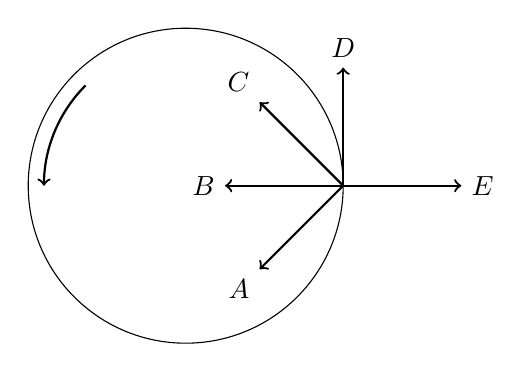
\begin{tikzpicture}
        %% Path
        \draw (0,0) circle (2cm);
        \draw[thick,->] (135:1.8) arc (135:180:1.8);
        %% Vectors
        \draw[thick,->] (2,0) -- ++ (90:1.5) node[anchor=south] {$D$};
        \draw[thick,->] (2,0) -- ++ (0:1.5) node[anchor=west] {$E$};
        \draw[thick,->] (2,0) -- ++ (135:1.5) node[anchor=south east] {$C$};
        \draw[thick,->] (2,0) -- ++ (180:1.5) node[anchor=east] {$B$};
        \draw[thick,->] (2,0) -- ++ (225:1.5) node[anchor=north east] {$A$};
    \end{tikzpicture}
    \end{center}
    Which arrow best depicts the net force acting on the object at the instant shown?
    \begin{multicols}{3}
    \begin{choices}[o]
        \wrongchoice{$A$}
      \correctchoice{$B$}
        \wrongchoice{$C$}
        \wrongchoice{$D$}
        \wrongchoice{$E$}
    \end{choices}
    \end{multicols}
\end{question}
}

\element{aapt}{ %% Bowl-A3
\begin{question}{bowl-1995-q06}
    The ``reaction'' force does not cancel the ``action'' force because:
    \begin{choices}
        \wrongchoice{The action force is greater than the reaction force.}
        \wrongchoice{The action force is less than the reaction force.}
      \correctchoice{They act on different bodies.}
        \wrongchoice{They are in the same direction.}
        \wrongchoice{The reaction exists only after the action force is removed.}
    \end{choices}
\end{question}
}

\element{aapt}{ %% Bowl-A3
\begin{question}{bowl-1995-q08}
    How long must a \SI{100}{\newton} net force act to produce a change in momentum of \SI{200}{\kilo\gram\meter\per\second}?
    \begin{multicols}{3}
    \begin{choices}
        \wrongchoice{\SI{0.25}{\second}}
        \wrongchoice{\SI{0.50}{\second}}
        \wrongchoice{\SI{1.0}{\second}}
      \correctchoice{\SI{2.0}{\second}}
        \wrongchoice{\SI{4.0}{\second}}
    \end{choices}
    \end{multicols}
\end{question}
}

\element{aapt}{ %% Bowl-A3
\begin{question}{bowl-1995-q34}
    A student pulls a wooden box along a rough horizontal floor at constant speed by means of a force $P$ as shown below.
    \begin{center}
    \begin{tikzpicture}
        %% Floor
        \node[anchor=north,fill,pattern=north east lines,minimum width=6cm, minimum height=0.05cm] at (0,0) {};
        \draw (-3,0) -- (3,0);
        %% Block
        \node[draw,fill=white!80!black,rectangle,rounded corners=1ex,minimum size=1.414cm,anchor=south] (M) at (0,0) {};
        %% Forces
        \draw[thick,->] (M.north) -- ++(90:1.5cm) node[anchor=north west] {$N$};
        \draw[thick,->] (M.west) -- ++(180:1.5cm) node[anchor=south west] {$f$};
        \draw[thick,->] (M.south) -- ++(270:1.5cm) node[anchor=south west] {$W$};
        \draw[dashed] (M.east) -- ++(0:1.5cm);
        \draw[<->] (M.east) ++ (0:0.75) arc(0:30:0.75) node[anchor=west,pos=0.5] {$\theta$};
        \draw[thick,->] (M.east) -- ++(30:1.5cm) node[anchor=south east] {$P$};
    \end{tikzpicture}
    \end{center}
    Which of the following must be true?
    \begin{multicols}{2}
    \begin{choices}
      \correctchoice{$P > f$ and $N < W$.}
        \wrongchoice{$P > f$ and $N = W$.}
        \wrongchoice{$P = f$ and $N > W$.}
        \wrongchoice{$P = f$ and $N = W$.}
        \wrongchoice{$P < f$ and $N = W$.}
    \end{choices}
    \end{multicols}
\end{question}
}

\element{aapt}{ %% Bowl-A3
\begin{question}{bowl-1995-q38}
    A block with initial velocity \SI{4.0}{\meter\per\second} slides \SI{8.0}{\meter} across a rough horizontal floor before coming to rest.
    The coefficient of friction is:
    \begin{multicols}{3}
    \begin{choices}
        \wrongchoice{\num{0.80}}
        \wrongchoice{\num{0.40}}
        \wrongchoice{\num{0.20}}
      \correctchoice{\num{0.10}}
        \wrongchoice{\num{0.05}}
    \end{choices}
    \end{multicols}
\end{question}
}


%% PhysicsBowl 1994
%%----------------------------------------
\element{aapt}{ %% Bowl-A3
\begin{question}{bowl-1994-q04}
    Newton's First Law is based in part on the work of:
    \begin{multicols}{3}
    \begin{choices}
        \wrongchoice{Dalton}
        \wrongchoice{Davy}
      \correctchoice{Galileo}
        \wrongchoice{Joule}
        \wrongchoice{Young}
    \end{choices}
    \end{multicols}
\end{question}
}

\element{aapt}{ %% Bowl-A3
\begin{question}{bowl-1994-q15}
    A car is traveling on a road in hilly terrain, see figure below.
    \begin{center}
    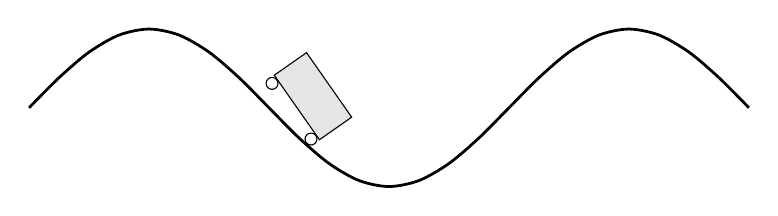
\begin{tikzpicture}[x=0.08\linewidth]
        %% sin curve
        \draw[domain=0:3*pi,smooth,line width=1pt] plot (\x, {sin(\x r)});
        %% cart at \pi radians
        \node[draw,fill=white!90!black,anchor=south,rotate=-55,minimum width=1cm,minimum height=0.5cm] (A) at (3.5,0) {};
        \draw (A.south west) ++(260:0.707ex) circle (0.5ex);
        \draw (A.south east) ++(170:0.707ex) circle (0.5ex);
    \end{tikzpicture}
    \end{center}
    Assume the car has speed $v$ and the tops and bottoms
        of the hills have radius of curvature $R$.
    The driver of the car is most likely to feel weightless:
    \begin{choices}
      \correctchoice{at the top of a hill when $v>\sqrt{gR}$.}
        \wrongchoice{at the bottom of a hill when $v>\sqrt{gR}$.}
        \wrongchoice{going down a hill when $v=\sqrt{gR}$.}
        \wrongchoice{at the top of a hill when $v<\sqrt{gR}$.}
        \wrongchoice{at the bottom of a hill when $v<\sqrt{gR}$.}
    \end{choices}
\end{question}
}

\element{aapt}{ %% Bowl-A3
\begin{question}{bowl-1994-q16}
    A car of mass $m$, traveling at speed $v$,
        stops in time $t$ when maximum braking force is applied.
    Assuming the braking force is independent of mass,
        what time would be required to stop a car of mass $2m$ traveling at speed $v$?
    \begin{multicols}{3}
    \begin{choices}
        \wrongchoice{$\dfrac{t}{2}$}
        \wrongchoice{$t$}
        \wrongchoice{$\sqrt{2}t$}
      \correctchoice{$2t$}
        \wrongchoice{$4t$}
    \end{choices}
    \end{multicols}
\end{question}
}

\element{aapt}{ %% Bowl-A3
\begin{question}{bowl-1994-q25}
    One end of a massless rope is attached to a mass $m$;
        the other end is attached to a mass of \SI{1.00}{\kilo\gram}.
    The rope is hung over a massless frictionless pulley as shown in the accompanying figure.
    \begin{center}
    \begin{tikzpicture}
        %% Ceiling
        \node[anchor=south,fill,pattern=north east lines,minimum width=4cm, minimum height=0.05cm] at (0,0) {};
        \draw (-2,0) -- (2,0);
        %% Pulley
        \draw (0,-1) circle (0.75);
        \draw[fill=white!90!black] (-0.3,0) -- (-0.2,-1.1) arc(190:350:0.2) -- (0.3,0) --cycle;
        \draw[fill] (0,-1) circle (1.5pt);
        %% Masses
        \node[draw,fill=white!90!black,rectangle,rounded corners=1ex,minimum size=1cm,anchor=north] (A) at (-0.75,-4) {$m$};
        \node[draw,fill=white!90!black,rectangle,rounded corners=1ex,minimum size=1cm,anchor=north] (B) at (0.75,-3) {\SI{1.0}{\kilo\gram}};
        %% Rope
        \draw[thick] (A.north) -- (-0.75,-1.0) arc(180:0:0.75) -- (B.north);
    \end{tikzpicture}
    \end{center}
    Mass $m$ accelerates downward at \SI{5.0}{\meter\per\second\squared}.
    What is $m$?
    \begin{multicols}{3}
    \begin{choices}
      \correctchoice{\SI{3.0}{\kilo\gram}}
        \wrongchoice{\SI{2.0}{\kilo\gram}}
        \wrongchoice{\SI{1.5}{\kilo\gram}}
        \wrongchoice{\SI{1.0}{\kilo\gram}}
        \wrongchoice{\SI{0.5}{\kilo\gram}}
    \end{choices}
    \end{multicols}
\end{question}
}

\element{aapt}{ %% Bowl-A3
\begin{question}{bowl-1994-q26}
    As shown in the accompanying figure, a force $F$ is exerted at an angle of $\theta$.
    \begin{center}
    \begin{tikzpicture}
        %% Floor
        \draw (-2,0) -- (2,0);
        \node[anchor=north,fill,pattern=north east lines,minimum width=4cm, minimum height=0.05cm] at (0,0) {};
        %% Box
        \node[fill=white!90!black,draw,anchor=south,minimum size=1.5cm] (A) at (-1,0) {};
        %% Force 
        \draw[thick,<-] (A.north east) -- ++(45:2) node[pos=0.5,anchor=south,rotate=45] {$F$};
        \draw[dashed] (A.north east) -- ++(0:1.33);
        \draw[<->] (A.north east) ++(0:1) arc (0:45:1) node[pos=0.5,anchor=west] {$\theta$};
        %% velocity
        \draw[thick,->] (0.5,0.5) -- ++(0:2) node[pos=0.5,anchor=south] {$v$};
    \end{tikzpicture}
    \end{center}
    The block of weight $mg$ is initially moving the right with speed $v$.
    The coefficient of friction between the rough floor and the block is $\mu$.
    The frictional force acting on the block is:
    \begin{choices}
        \wrongchoice{$\mu mg$ to the right}
        \wrongchoice{$\mu mg$ to the left}
        \wrongchoice{$\mu mg - F\sin\theta$ to the left}
        \wrongchoice{$\mu\left( mg - F\sin\theta\right)$ to the right}
      \correctchoice{$\mu\left( mg + F\sin\theta\right)$ to the left}
    \end{choices}
\end{question}
}


\endinput


